% !TeX program = xelatex
\documentclass{article}
\usepackage{kotex}
\usepackage[a4paper,left=3cm, right=3cm, top=2cm, bottom=2cm]{geometry}
\usepackage{amsmath}
\usepackage{graphicx}
\usepackage{caption}
\usepackage{setspace}
\usepackage{xcolor}
\usepackage{titlesec}
\usepackage{amssymb}
\usepackage{tcolorbox}
\usepackage{amsthm}
\usepackage{multirow}
\usepackage{array}
\usepackage{booktabs}
\usepackage{tikz}
\usetikzlibrary{positioning,arrows.meta,calc,shapes.geometric}
\usepackage{cancel}
\usepackage{pgfplots}
\pgfplotsset{compat=1.18}

\title{9.1 \textit{LU}-Decompositions}
\date{}
\author{}
\setstretch{1.3}

\titleformat{name=\section, numberless}
  {\normalfont\large\bfseries\color{blue}}{}
  {0pt}{}
\geometry{a4paper, margin=1in}

\newcommand{\redheading}[1]{{\vspace{2mm}\noindent\Large\bfseries\color{red!55!black} #1\par}\vspace{2mm}}

\begin{document}
\maketitle

{\itshape\color{blue!45!black}
Up to now, we have focused on Gaussian elimination and Gauss--Jordan elimination for
solving linear systems. While suitable for small problems, these methods are not ideal
for large-scale problems where computer roundoff error, memory, and speed are concerns.
In this section we discuss a method based on factoring the coefficient matrix into a
product of lower and upper triangular matrices---the \emph{LU-decomposition}---which
underpins many computer algorithms.\par}

\vspace{2mm}

\redheading{Solving Linear Systems by Factoring}

Our first goal is to show how to solve $A\mathbf{x} = \mathbf{b}$ (an $n\times n$
system) by factoring the coefficient matrix $A$.

\begin{tcolorbox}[colback=teal!4, colframe=teal!65!black,
  title={\textbf{Definition 1}}, boxrule=0.5mm, arc=3mm]
A factorization of a square matrix $A$ as
\[
  A = LU \tag{1}
\]
where $L$ is lower triangular and $U$ is upper triangular is called an
\textbf{\textit{LU}-decomposition} (or \textbf{\textit{LU}-factorization}) of $A$.
\end{tcolorbox}

\begin{tcolorbox}[colback=blue!4, colframe=blue!55!black,
  title={\textbf{The Method of \textit{LU}-Decomposition}}, boxrule=0.5mm, arc=3mm]
\textbf{Step 1.} Rewrite $A\mathbf{x} = \mathbf{b}$ as
\[
  LU\mathbf{x} = \mathbf{b} \tag{2}
\]
\textbf{Step 2.} Substitute $\mathbf{y} = U\mathbf{x}$ and rewrite (2) as
$L\mathbf{y} = \mathbf{b}$; solve for $\mathbf{y}$ (\emph{forward substitution}).

\textbf{Step 3.} Substitute $\mathbf{y}$ into $U\mathbf{x} = \mathbf{y}$ and solve for
$\mathbf{x}$ (\emph{back substitution}).
\end{tcolorbox}

This procedure replaces the single system $A\mathbf{x} = \mathbf{b}$ by the two
triangular systems $L\mathbf{y} = \mathbf{b}$ and $U\mathbf{x} = \mathbf{y}$, which are
solved in succession. Because each system has a triangular coefficient matrix, the total
computation is generally no more than solving the original system directly.

\begin{figure}[ht]
\centering
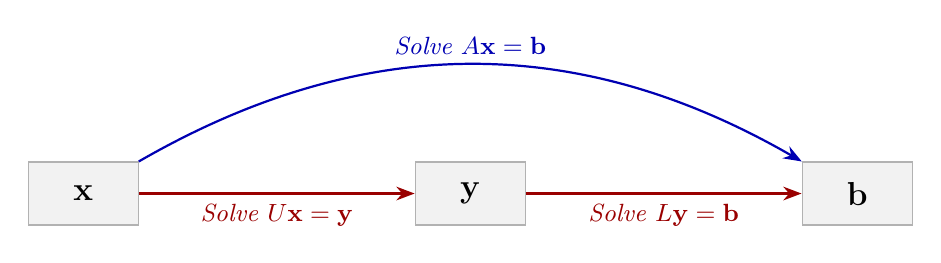
\begin{tikzpicture}[>=Stealth, node distance=3.2cm]
  \node[draw=gray!60, fill=gray!10, minimum width=1.4cm, minimum height=0.8cm,
        inner sep=4pt, font=\large\bfseries] (x) {$\mathbf{x}$};
  \node[draw=gray!60, fill=gray!10, minimum width=1.4cm, minimum height=0.8cm,
        inner sep=4pt, font=\large\bfseries, right=3.5cm of x] (y) {$\mathbf{y}$};
  \node[draw=gray!60, fill=gray!10, minimum width=1.4cm, minimum height=0.8cm,
        inner sep=4pt, font=\large\bfseries, right=3.5cm of y] (b) {$\mathbf{b}$};
  \draw[->, thick, blue!70!black]
    (x) to[bend left=30]
    node[above, font=\small\itshape]{Solve $A\mathbf{x}=\mathbf{b}$} (b);
  \draw[->, thick, red!60!black]
    (x) -- node[below, font=\small\itshape]{Solve $U\mathbf{x}=\mathbf{y}$} (y);
  \draw[->, thick, red!60!black]
    (y) -- node[below, font=\small\itshape]{Solve $L\mathbf{y}=\mathbf{b}$} (b);
\end{tikzpicture}
\caption*{FIGURE 9.1.1}
\end{figure}

\subsection*{EXAMPLE 1 | Solving $A\mathbf{x} = \mathbf{b}$ by \textit{LU}-Decomposition}

Use the \textit{LU}-decomposition
\[
  \begin{bmatrix}2&6&2\\-3&-8&0\\4&9&2\end{bmatrix}
  = \underbrace{\begin{bmatrix}2&0&0\\-3&1&0\\4&-3&7\end{bmatrix}}_{L}
    \underbrace{\begin{bmatrix}1&3&1\\0&1&3\\0&0&1\end{bmatrix}}_{U} \tag{4}
\]
to solve the system
$\begin{bmatrix}2&6&2\\-3&-8&0\\4&9&2\end{bmatrix}
\begin{bmatrix}x_1\\x_2\\x_3\end{bmatrix}
=\begin{bmatrix}2\\2\\3\end{bmatrix}$.

\textbf{SOLUTION:} Rewriting as $LU\mathbf{x}=\mathbf{b}$ and setting $\mathbf{y}=U\mathbf{x}$, we first solve $L\mathbf{y}=\mathbf{b}$:
\[
  \begin{bmatrix}2&0&0\\-3&1&0\\4&-3&7\end{bmatrix}
  \begin{bmatrix}y_1\\y_2\\y_3\end{bmatrix}
  =\begin{bmatrix}2\\2\\3\end{bmatrix}
  \quad\Longrightarrow\quad
  \begin{aligned}
    2y_1 &= 2\\
    -3y_1 + y_2 &= 2\\
    4y_1 - 3y_2 + 7y_3 &= 3
  \end{aligned}
\]
Forward substitution gives $y_1=1,\ y_2=5,\ y_3=2$.
Substituting into $U\mathbf{x}=\mathbf{y}$:
\[
  \begin{bmatrix}1&3&1\\0&1&3\\0&0&1\end{bmatrix}
  \begin{bmatrix}x_1\\x_2\\x_3\end{bmatrix}
  =\begin{bmatrix}1\\5\\2\end{bmatrix}
  \quad\Longrightarrow\quad
  \begin{aligned}
    x_1+3x_2+x_3 &= 1\\
    x_2+3x_3 &= 5\\
    x_3 &= 2
  \end{aligned}
\]
Back substitution yields $x_1=2,\ x_2=-1,\ x_3=2$.

\vspace{2mm}
\redheading{Finding \textit{LU}-Decompositions}

Once an $LU$-decomposition of $A$ is found, solving a sequence of systems
$A\mathbf{x}=\mathbf{b}_1,\,A\mathbf{x}=\mathbf{b}_2,\,\ldots,\,A\mathbf{x}=\mathbf{b}_k$
requires factoring $A$ only once; the factorization is then reused for each right-hand side.
This is the main advantage of $LU$-decomposition.

Not every square matrix has an $LU$-decomposition. However, if $A$ can be reduced to
row echelon form by Gaussian elimination \emph{without row interchanges}, then it has one.
Specifically, if elementary matrices $E_1,E_2,\ldots,E_k$ (none involving row
interchanges) reduce $A$ to $U$, so that
\[
  E_k\cdots E_2 E_1 A = U \tag{8}
\]
then $A = E_1^{-1}E_2^{-1}\cdots E_k^{-1}U = LU$, where
\[
  L = E_1^{-1}E_2^{-1}\cdots E_k^{-1} \tag{10}
\]

\begin{tcolorbox}[colback=red!4, colframe=red!60!black,
  title={\textbf{Theorem 9.1.1}}, boxrule=0.5mm, arc=3mm]
If $A$ is a square matrix that can be reduced to row echelon form $U$ by Gaussian
elimination without row interchanges, then $A$ can be factored as $A = LU$, where $L$
is lower triangular.
\end{tcolorbox}

\textit{Proof.}
Let $L$ and $U$ be as in Formulas (10) and (8). $U$ is upper triangular because it is
a row echelon form of a square matrix. Each $E_j$ (no row interchange) either adds a
scalar multiple of one row to a lower row, or scales a row by a nonzero constant; in both
cases $E_j$ is lower triangular, and by Theorem~1.7.1(d) so is $E_j^{-1}$. Hence $L$,
a product of lower triangular matrices, is lower triangular. $\blacksquare$

\subsection*{EXAMPLE 2 | An \textit{LU}-Decomposition}

Find an $LU$-decomposition of
$A = \begin{bmatrix}2&6&2\\-3&-8&0\\4&9&2\end{bmatrix}$.

\textbf{SOLUTION:} We reduce $A$ to row echelon form without row interchanges and track
the elementary matrices and their inverses.

\renewcommand{\arraystretch}{1.1}
\begin{center}
\begin{tabular}{|l|l|l|l|}
\hline
\textbf{Reduction step} & \textbf{Row op} & $E_j$ & $E_j^{-1}$ \\
\hline
Step 1: $\frac{1}{2}\times$row~1 &
$\frac{1}{2}r_1$&
$\begin{bmatrix}\frac{1}{2}&0&0\\0&1&0\\0&0&1\end{bmatrix}$&
$\begin{bmatrix}2&0&0\\0&1&0\\0&0&1\end{bmatrix}$ \\
\hline
Step 2: $3r_1+r_2$ &
$(3\!\times\!r_1)+r_2$&
$\begin{bmatrix}1&0&0\\3&1&0\\0&0&1\end{bmatrix}$&
$\begin{bmatrix}1&0&0\\-3&1&0\\0&0&1\end{bmatrix}$ \\
\hline
Step 3: $-4r_1+r_3$ &
$(-4\!\times\!r_1)+r_3$&
$\begin{bmatrix}1&0&0\\0&1&0\\-4&0&1\end{bmatrix}$&
$\begin{bmatrix}1&0&0\\0&1&0\\4&0&1\end{bmatrix}$ \\
\hline
Step 4: $3r_2+r_3$ &
$(3\!\times\!r_2)+r_3$&
$\begin{bmatrix}1&0&0\\0&1&0\\0&3&1\end{bmatrix}$&
$\begin{bmatrix}1&0&0\\0&1&0\\0&-3&1\end{bmatrix}$ \\
\hline
Step 5: $\frac{1}{7}\times$row~3 &
$\frac{1}{7}r_3$&
$\begin{bmatrix}1&0&0\\0&1&0\\0&0&\frac{1}{7}\end{bmatrix}$&
$\begin{bmatrix}1&0&0\\0&1&0\\0&0&7\end{bmatrix}$ \\
\hline
\end{tabular}
\end{center}

The result is $U = \begin{bmatrix}1&3&1\\0&1&3\\0&0&1\end{bmatrix}$, and computing
$L = E_1^{-1}E_2^{-1}E_3^{-1}E_4^{-1}E_5^{-1}$ yields
\[
  L = \begin{bmatrix}2&0&0\\-3&1&0\\4&-3&7\end{bmatrix} \tag{11}
\]
so $A = LU$ agrees with the factorization in Example~1.

\vspace{2mm}
\redheading{Bookkeeping}

The matrix computation in Example~2 is unnecessary. Observe:
\begin{itemize}
  \item The \textbf{diagonal entries} of $L$ are the reciprocals of the multipliers used
        to introduce leading 1's in $U$.
  \item Each \textbf{off-diagonal entry} of $L$ below the main diagonal is the
        \emph{negative} of the multiplier used to introduce the zero in that position in $U$.
\end{itemize}
This gives a streamlined 4-step procedure:

\begin{tcolorbox}[colback=blue!4, colframe=blue!55!black,
  title={\textbf{Procedure for Constructing an \textit{LU}-Decomposition}},
  boxrule=0.5mm, arc=3mm]
\textbf{Step 1.} Reduce $A$ to row echelon form $U$ by Gaussian elimination without row
interchanges, tracking the multipliers for each leading~1 and each zero introduced below
a leading~1.

\textbf{Step 2.} Along the main diagonal of $L$, place the \emph{reciprocal} of each
multiplier that introduced a leading~1 in $U$.

\textbf{Step 3.} At each position below the main diagonal of $L$, place the
\emph{negative} of the multiplier used to introduce the zero at that position in $U$.

\textbf{Step 4.} Form the decomposition $A = LU$.
\end{tcolorbox}

\subsection*{EXAMPLE 3 | Constructing an \textit{LU}-Decomposition}

Find an $LU$-decomposition of $A = \begin{bmatrix}6&-2&0\\9&-1&1\\3&7&5\end{bmatrix}$.

\textbf{SOLUTION:} We reduce $A$ to $U$ while filling in $L$ simultaneously (bullets
denote not-yet-determined entries of $L$).

\[
A = \begin{bmatrix}6&-2&0\\9&-1&1\\3&7&5\end{bmatrix},\qquad
L = \begin{bmatrix}\bullet&0&0\\\bullet&\bullet&0\\\bullet&\bullet&\bullet\end{bmatrix}
\]

\noindent\textit{Step 1:} $\frac{1}{6}\times r_1$ (multiplier $= \frac{1}{6}$, so $l_{11}=6$):
\[
\begin{bmatrix}1&-\frac{1}{3}&0\\9&-1&1\\3&7&5\end{bmatrix},\qquad
L_{11}=6
\]

\noindent\textit{Step 2:} $(-9)\times r_1 + r_2$ and $(-3)\times r_1 + r_3$ (multipliers
$-9$ and $-3$, so $l_{21}=9,\,l_{31}=3$):
\[
\begin{bmatrix}1&-\frac{1}{3}&0\\0&2&1\\0&8&5\end{bmatrix},\qquad
L=\begin{bmatrix}6&0&0\\9&\bullet&0\\3&\bullet&\bullet\end{bmatrix}
\]

\noindent\textit{Step 3:} $\frac{1}{2}\times r_2$ (multiplier $=\frac{1}{2}$, so $l_{22}=2$):
\[
\begin{bmatrix}1&-\frac{1}{3}&0\\0&1&\frac{1}{2}\\0&8&5\end{bmatrix},\qquad
L_{22}=2
\]

\noindent\textit{Step 4:} $(-8)\times r_2 + r_3$ (multiplier $-8$, so $l_{32}=8$):
\[
\begin{bmatrix}1&-\frac{1}{3}&0\\0&1&\frac{1}{2}\\0&0&1\end{bmatrix},\qquad
L=\begin{bmatrix}6&0&0\\9&2&0\\3&8&\bullet\end{bmatrix}
\]

\noindent\textit{Step 5:} $r_3$ already has leading~1 (multiplier $=1$, so $l_{33}=1$):
\[
U = \begin{bmatrix}1&-\frac{1}{3}&0\\0&1&\frac{1}{2}\\0&0&1\end{bmatrix},\qquad
L = \begin{bmatrix}6&0&0\\9&2&0\\3&8&1\end{bmatrix}
\]
Thus the $LU$-decomposition is
\[
  \begin{bmatrix}6&-2&0\\9&-1&1\\3&7&5\end{bmatrix}
  = \begin{bmatrix}6&0&0\\9&2&0\\3&8&1\end{bmatrix}
    \begin{bmatrix}1&-\frac{1}{3}&0\\0&1&\frac{1}{2}\\0&0&1\end{bmatrix}
\]

\vspace{2mm}
\redheading{\textit{LU}-Decompositions Are Not Unique}

In general, $LU$-decompositions are not unique. If $A = LU$ and $L$ has nonzero diagonal
entries (guaranteed when $A$ is invertible), we can shift diagonal entries from $L$ to a
separate diagonal matrix $D$, writing $L = L'D$ where $L'$ has 1's on the main diagonal.
This gives another $LU$-decomposition $A = (L')(DU)$.

\vspace{2mm}
\redheading{\textit{LDU}-Decompositions}

If it is preferred to have 1's on the main diagonal of \emph{both} the lower and upper
triangular factors, we can factor as $L = L'D$ and write
\[
  A = L'DU
\]
where $L'$ has 1's on the diagonal, $D$ is diagonal, and $U$ has 1's on the diagonal.
This is the \textbf{\textit{LDU}-decomposition} of $A$. For example,
\[
  \begin{bmatrix}2&6&2\\-3&-8&0\\4&9&2\end{bmatrix}
  = \begin{bmatrix}1&0&0\\-\frac{3}{2}&1&0\\2&-3&1\end{bmatrix}
    \begin{bmatrix}2&0&0\\0&1&0\\0&0&7\end{bmatrix}
    \begin{bmatrix}1&3&1\\0&1&3\\0&0&1\end{bmatrix} \tag{13}
\]
If $A$ is invertible and can be reduced to row echelon form without row interchanges,
then $A$ can be factored \emph{uniquely} as $A = LDU$.

\vspace{2mm}

\section*{Exercise Set 9.1}

\noindent\textit{In Exercises 1--2, use the given LU-decomposition to solve the system.}

\begin{enumerate}
  \item $\begin{bmatrix}3&-6\\-2&5\end{bmatrix}
        = \begin{bmatrix}3&0\\-2&1\end{bmatrix}
          \begin{bmatrix}1&-2\\0&1\end{bmatrix}$;\quad
        solve $3x_1 - 6x_2 = 0$,\; $-2x_1 + 5x_2 = 1$.

  \item $\begin{bmatrix}3&-6&-3\\2&0&6\\-4&7&4\end{bmatrix}
        = \begin{bmatrix}3&0&0\\2&4&0\\-4&-1&2\end{bmatrix}
          \begin{bmatrix}1&-2&-1\\0&1&2\\0&0&1\end{bmatrix}$;\quad
        solve $3x_1-6x_2-3x_3=-3$,\; $2x_1+6x_3=-22$,\; $-4x_1+7x_2+4x_3=3$.

\end{enumerate}

\noindent\textit{In Exercises 3--6, find an LU-decomposition of the coefficient matrix
and then use the method of Example~1 to solve the system.}

\begin{enumerate}
  \item[3.] $\begin{bmatrix}2&8\\-1&-1\end{bmatrix}
             \begin{bmatrix}x_1\\x_2\end{bmatrix}
             = \begin{bmatrix}-2\\-2\end{bmatrix}$

  \item[5.] $\begin{bmatrix}2&-2&-2\\0&-2&2\\-1&5&2\end{bmatrix}
             \begin{bmatrix}x_1\\x_2\\x_3\end{bmatrix}
             = \begin{bmatrix}-4\\-2\\6\end{bmatrix}$

\end{enumerate}

\noindent\textit{In Exercises 7--8, an LU-decomposition of $A$ is given.}

\textbf{a.} Compute $L^{-1}$ and $U^{-1}$.

\textbf{b.} Use the result in part (a) to find the inverse of $A$.

\begin{enumerate}
  \item[7.] $A = \begin{bmatrix}2&-1&3\\4&2&1\\-6&-1&2\end{bmatrix}$;\quad
        $A = LU = \begin{bmatrix}1&0&0\\2&1&0\\-3&-1&1\end{bmatrix}
                  \begin{bmatrix}2&-1&3\\0&4&-5\\0&0&6\end{bmatrix}$

\end{enumerate}

\noindent\textit{Exercise 9.} Let
$A = \begin{bmatrix}2&1&-1\\-2&-1&2\\2&1&0\end{bmatrix}$.

\textbf{a.} Find an $LU$-decomposition of $A$.

\textbf{b.} Express $A$ in the form $A = L_1 D U_1$, where $L_1$ is lower triangular
with 1's along the main diagonal, $U_1$ is upper triangular with 1's along the main
diagonal, and $D$ is a diagonal matrix.

\textbf{c.} Express $A$ in the form $A = L_2 U_2$, where $L_2$ is lower triangular
with 1's along the main diagonal and $U_2$ is upper triangular.

\begin{enumerate}
  \item[10.] \textbf{a.} Show that the matrix
        $\begin{bmatrix}0&1\\1&0\end{bmatrix}$ has no $LU$-decomposition.

        \textbf{b.} Find a $PLU$-decomposition of this matrix.

\end{enumerate}

\noindent\textit{In Exercises 11--12, use the given PLU-decomposition of $A$ to solve
$A\mathbf{x}=\mathbf{b}$ by rewriting it as $P^{-1}A\mathbf{x}=P^{-1}\mathbf{b}$
and solving by LU-decomposition.}

\begin{enumerate}
  \item[12.] $\mathbf{b} = \begin{bmatrix}3\\0\\6\end{bmatrix}$;\quad
        $A = \begin{bmatrix}4&1&2\\0&2&1\\8&1&8\end{bmatrix}$;\quad
        $A = \underbrace{\begin{bmatrix}0&0&1\\0&1&0\\1&0&0\end{bmatrix}}_{P}
             \underbrace{\begin{bmatrix}1&0&0\\0&1&0\\\frac{1}{2}&\frac{1}{4}&1\end{bmatrix}}_{L}
             \underbrace{\begin{bmatrix}8&1&8\\0&2&1\\0&0&-\frac{9}{4}\end{bmatrix}}_{U} = PLU$

\end{enumerate}

\noindent\textit{In Exercises 13--14, find the LDU-decomposition of $A$.}

\begin{enumerate}
  \item[13.] $A = \begin{bmatrix}2&2\\4&1\end{bmatrix}$

  \item[14.] $A = \begin{bmatrix}3&-12&6\\0&2&0\\6&-28&13\end{bmatrix}$

\end{enumerate}

\noindent\textit{In Exercises 15--16, find a PLU-decomposition of $A$, and use it to
solve $A\mathbf{x}=\mathbf{b}$.}

\begin{enumerate}
  \item[16.] $A = \begin{bmatrix}0&3&-2\\1&1&4\\2&2&5\end{bmatrix}$;\quad
        $\mathbf{b} = \begin{bmatrix}7\\5\\-2\end{bmatrix}$

\end{enumerate}

\noindent\textit{Working with Proofs}

\begin{enumerate}
  \item[17.] Let $A\mathbf{x}=\mathbf{b}$ be a linear system of $n$ equations in $n$
        unknowns, and assume $A$ is invertible and can be reduced to row echelon form
        without row interchanges. How many additions and multiplications are required to
        solve the system by the method of Example~1?

\end{enumerate}

\end{document}
